\documentclass[12pt]{report}

%\usepackage{enumitem}
\usepackage{indentfirst}
\usepackage{graphicx}
\usepackage[labelfont=bf,justification=justified,singlelinecheck=false]{caption}

\usepackage{tocloft}
\usepackage{caption}
\usepackage{enumerate}
\usepackage[cal=boondoxo]{mathalfa}
\usepackage{courier}
\usepackage[hidelinks]{hyperref}

\usepackage{amsmath}
\usepackage{amsthm}
\usepackage{amssymb}
\usepackage{cite}
\usepackage[mathscr]{euscript}

\usepackage{algorithm}
\usepackage{algpseudocode}
\usepackage{verbatim}


\setcounter{secnumdepth}{5}
\setcounter{tocdepth}{3}


\newtheorem{prop}{Proposition}
\newtheorem{lemma}{Lemma}
\newtheorem{corollary}{Corollary}
\newtheorem{property}{Property}

\renewcommand{\bibname}{References}

\usepackage{color}


\title{AVDTA: Dynamic Traffic Assignment}
\author{Michael W. Levin}

\begin{document}
	\allowdisplaybreaks
	\pagenumbering{gobble}
	
	\maketitle
	\newpage
	
	
	
	
	
	\pagenumbering{roman}
	
	\renewcommand*\contentsname{Table of Contents}
	\tableofcontents
	\newpage
	
	\pagenumbering{arabic}
	
	
	% Introduction
	% 	Organization
	\chapter{Introduction}





\section*{Distribution}
AVDTA is a research software for studying DTA and mesoscopic simulation models of autonomous vehicle technologies. AVDTA is not available for commercial use. AVDTA may not be used without the permission of the author, \theauthor.


\section*{Support}
The author may be contacted at \href{mailto:michaellevin@utexas.edu}{michaellevin@utexas.edu}.
	
	%Project - definition
	% 	File structure
	%	Options
	\chapter{Project structure}


\section{Introduction}

AVDTA is organized around \textit{projects}. A project is best thought of as a specific scenario under study. For instance, a project might represent a certain demand scenario or network configuration for a city network or subnetwork. The AVDTA GUI contains methods to modify project options, such as link types or intersection controls. Data files can also be copied to and from Excel for easy modification.

\section{GUI}

The AVDTA GUI is designed to interact with projects. Each instance of AVDTA can have a single project open at a time. Projects can be created and opened via the ``File'' menu.

\begin{center}
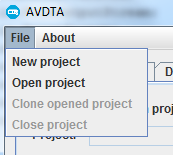
\includegraphics[scale=1]{images/project1.png}
\end{center}


\subsection{New project}
\label{sec:newproject}
To create a new project, you will first be asked to select the root folder. By default, this folder is \texttt{avdta/projects}, but it may be changed.

\begin{center}
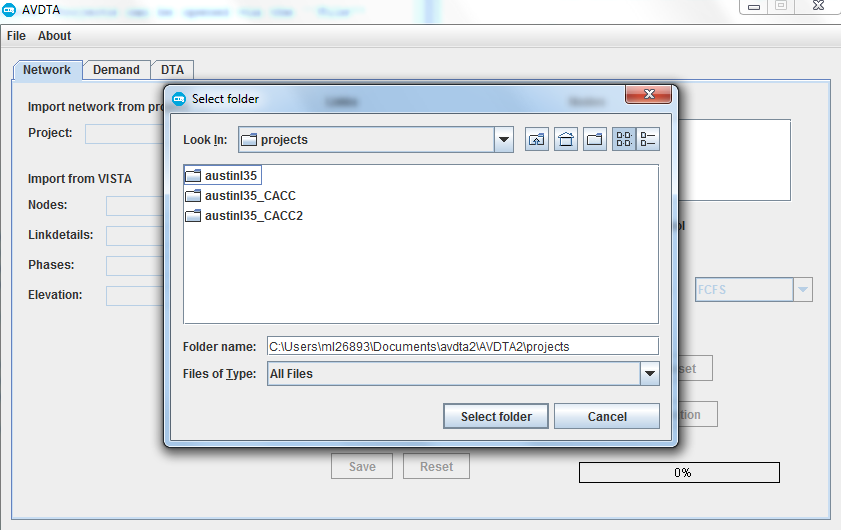
\includegraphics[width=0.8\textwidth]{images/project2.png}
\end{center}

You will then be asked to enter the name of the new project. A project folder with the entered name will be created in the selected root folder.


\begin{center}
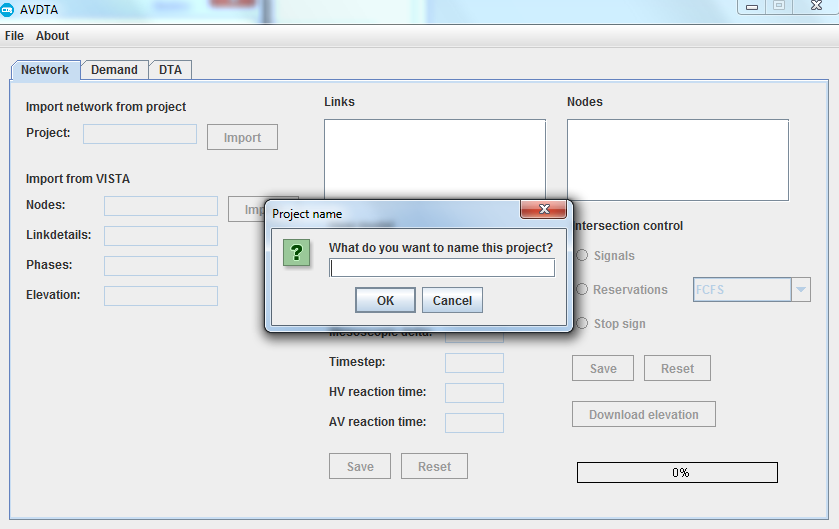
\includegraphics[width=0.8\textwidth]{images/project3.png}
\end{center}

\subsection{Open project}

AVDTA project folders are shown with a special icon. Select a project folder and click ``open project'' to open it.

\begin{center}
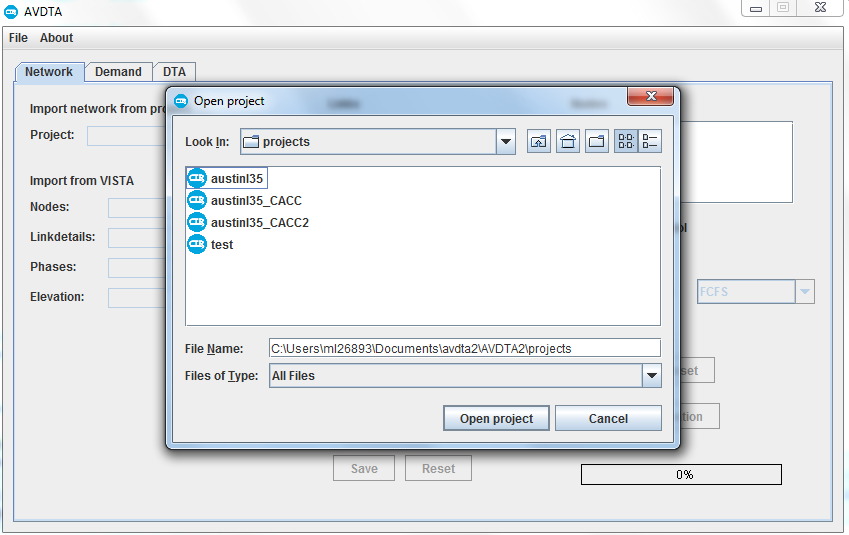
\includegraphics[width=0.8\textwidth]{images/project4.png}
\end{center}

\subsection{Clone opened project}

If a project is open, the AVDTA GUI enables the option of creating a clone. Follow the instructions in Section \ref{sec:newproject} to choose the location and name of the clone. You can also create a copy of a project folder within the file system.

\section{Files and folders}

A project consists of a file folder containing several specific files and subfolders. The project folder, along with many of its files and subfolders, is automatically generated when a new project is created. However, many files will be empty, requiring the import of data from other projects or other sources. Note that removal or modification of these files outside of the AVDTA GUI could result in errors when loading the project. However, adding files or folders will not affect the project. 

Projects contain several types of files. Text files (\texttt{.txt}) contain project inputs or outputs and are intended to be read or modified. However, if modifying these files, ensure that the format and units are correct. Text files are tab-delimited, and have a header indicating the data in each column. Text files may be copied to and from Excel.

Data files (\texttt{.dat}) are used to load the project and are not intended to be opened or modified. Similarly, files with other unknown extensions are not intended to be opened.

\subsection{Files}

\subsubsection{\texttt{project.txt}}
The \texttt{project.txt} file contains project properties used to load the project within AVDTA. The file consists of two columns:
 The file consists of two columns:
\begin{center}
\begin{tabular}{cc}
\hline
key & value\\\hline
\end{tabular}
\end{center}


\paragraph*{name}
This is the project name that is displayed when AVDTA loads a project. This does not have to correspond to the project folder name.

\paragraph*{seed}
This is the random number generator seed. If two projects have matching seeds, actions involving random numbers performed in the same order should have identical outputs.

\paragraph*{type}
This denotes the project type.


\subsubsection{\texttt{options.txt}}
The \texttt{options.txt} file contains project parameters that define the loading and simulation of the project. The file consists of two columns:
\begin{center}
\begin{tabular}{cc}
\hline
key & value\\\hline
\end{tabular}
\end{center}
Keys are case insensitive. Values are a string that could represent multiple data types, such as integers, floating-point numbers, or booleans (``true'' or ``false''). The options file is automatically generated with default values when a project is created. 

\paragraph*{av-reaction-time}
This is used to determine the capacity and congested wave speed increase due to autonomous vehicles when using the multiclass CTM~\cite{levin2016multiclass}. A typical value is 0.5 (s). Note that capacity and congested wave speed are scaled from the values in the \texttt{networks/links.txt} file.

\paragraph*{hv-reaction-time}
This is used to determine the baseline capacity and congested wave speed when using the multiclass CTM~\cite{levin2016multiclass}. A typical value is 1 (s). Note that capacity and congested wave speed are scaled from the values in the \texttt{networks/links.txt} file.

\paragraph*{dynamic-lane-reversal}
If set to ``true'', DLR will be activated on DLR links. DLR is a specific type of CTM link, and the type of links can be set in the \texttt{networks/links.txt} file.

\paragraph*{hvs-use-reservations}
If set to ``true'', HVs will not avoid reservation-controlled intersections in their route choices. Reservations will use the legacy early method for intelligent traffic management~\cite{conde2013intelligent}, adapted to DNL~\cite{levin2016multiclass} for HVs. Otherwise, HVs will avoid reservations in their route choices, passing through reservations only if no other route is available.

\paragraph*{simulation-duration}
This is the duration of the simulation, in seconds. The duration should be sufficiently longer than the demand departure times interval to allow all vehicles to exit the network.

\paragraph*{simulation-mesoscopic-step}
This is the time step used in simulation. For CTM, a typical value is 6 (s). For LTM, a typical value is 10 (s).

\paragraph*{ast-duration}
This the interval for averaging travel times for calculating shortest paths. A typical value is 900 (s).














	
	
	\chapter{Traffic network}
\label{ch:network}

%Network structure
%	Links
%	Nodes
%	Zones
%	Data files - include in each of the above section
%	GUI - include in each of the above sections
%	Import from VISTA
%	Types - include in each o the above sections

\section{Introduction}
A \textit{network} in AVDTA defines the road structure through which vehicles can flow. It does not include vehicular demand or trips because these depend on the application. For instance, the vehicle trips for DTA models is different from vehicle trips for SAV models. The network in AVDTA compartmentalizes the road network, with vehicle trips handled separately depending on the application.

A network consists of \textit{nodes} and (directed) \textit{links} connecting nodes. Nodes are further divided into \textit{intersections}, which connect roads, and \textit{zones}, where demand and vehicles can enter or exit the network. AVDTA includes several options for intersection controls and link flow models, which are discussed in Sections \ref{sec:nodes} and \ref{sec:links}, respectively. The discussion in this document pertains to using and modifying node and link data within AVDTA. References to the theoretical developments of flow models are included.

Network data files are contained in the \texttt{network} subfolder within a project folder. Network files include \texttt{nodes.txt}, \texttt{links.txt}, and \texttt{phases.txt} (which defines signal phases for nodes). All data files include a header as the first line. 

\section{Nodes}
\label{sec:nodes}

Nodes are either intersections or zones. Intersections represent physical intersections in the road network, and zones represent locations where vehicles or travelers enter and exit. It is typical for zones to double intersections. Each zone should be either a source or a sink.

Each node has sets of incoming and outgoing links. During simulation, nodes determine vehicle flow from incoming links to outgoing links. Incoming links define \textit{sending flows} as a set of vehicles, and outgoing links define \textit{receiving flows}. Vehicle flow is constrained by sending and receiving flows, and may be additionally constrained by intersection conflict constraints. 

\subsection{\texttt{nodes.txt}}
The \texttt{nodes.txt} file contains the data to describe intersections and zones, and consists of the following:
\begin{center}
\begin{tabular}{ccccc}
\hline
id & type & longitude & latitude  & elevation \\\hline
\end{tabular}
\end{center}
Columns are tab-delimited, and each line corresponds to a new node. Additional columns will be ignored, and may be deleted if the GUI is used to modify the file.

\paragraph*{id}
Each node must be given an unique id, which is used to identify the node in other data files. Ids should be positive, but do not need to be consecutive.

\paragraph*{type}
The type specifies whether the node is a zone or an intersection. If an intersection, the type also identifies the intersection control. Type options are given below.
\begin{center}
\begin{tabular}{lcl}
\hline
Category & Type & Description\\\hline
Reservations & 301 & FCFS\\
& 332 & Pressure-based\\
& 333 & $P_0$\\
& 334 & $Q^2$~\cite{levin2015optimizing}\\
& 335 & $DE^4$~\cite{levin2015optimizing}\\
& 321 & {\sc Phased}\\
& 322 & {\sc Weighted}\\\hline
Traffic signal & 100 & Standard traffic signal\\\hline
Stop sign & 200 & 4-way stop \\\hline
Centroid & 1000 & Centroid\\\hline
\end{tabular}
\end{center}
Note that merges and diverges will be automatically used. An intersection with only one incoming link will become a diverge, and an intersection with only one outgoing link will become a merge. This is because merges/diverges avoid the need for intersection controls, and also performed better than some reservation policies~\cite{levin2016paradoxes}.

\paragraph*{longitude/latitude}
Longitude and latitudes are specified in decimal format, with the sign indicating west/east and north/south, respectively. The longitude/latitude data is used only for display purposes. False data will not affect vehicle loading or simulation. Zones doubling an intersection typically have the same coordinates.

\paragraph*{elevation}
Elevation data is used to determine link grade for estimating vehicle fuel consumptions~\cite{levin2014effect}. False data will not affect vehicle loading or simulation. The GUI contains a method to download elevation data from Google Maps, given longitudes and latitudes.

\subsection{\texttt{phases.txt}}
The \texttt{phases.txt} file contains information about signal phases. Note that the order in which the phases appear is the order in which they will be created for the signal cycle. Each line in the \texttt{phases.txt} file is a separate phase, and the columns are
\begin{center}
\begin{tabular}{ccccccc}
\hline
id & nodeid & time\_red & time\_yellow & time\_green & num\_moves	link\_from & link\_to\\\hline
\end{tabular}
\end{center}
\paragraph*{id} The id for the phases. Ids do not have to be consecutive, but they must be unique and positive.
\paragraph*{nodeid} The node id for which the phase is valid.
\paragraph*{time\_red, time\_yellow} Clearance interval times for this phase.
\paragraph*{time\_green} Green time for this phase.
\paragraph*{num\_moves} The number of protected turning movements, also the size of the ``link\_from'' and ``link\_to'' arrays.
\paragraph*{link\_from, link\_to} Protected turning movements for this phase. These consist of two equal-length arrays, one of incoming links and one of outgoing links. A valid turning movement is a pair of an incoming link and an outgoing link. Consequently, links may appear multiple times in the arrays to enumerate all protected turning movements.

The \texttt{signals.txt} file contains signal offsets for each node. Each node may have one entry. Duplicate entries will overwrite previous ones. A missing entry indicates an offset of $0$. The \texttt{signals.txt} file columns are
\begin{center}
\begin{tabular}{cc}
\hline
nodeid & offset\\\hline
\end{tabular}
\end{center}
\paragraph*{nodeid} the node id for this signal
\paragraph*{offset} the time offset (in seconds). This can be a floating point number.


\subsection{GUI panel}

The AVDTA GUI nodes panel is on the right hand side of the ``network'' tab. The uppermost text area displays information about the network, including the number of total nodes, and nodes of each type.
\begin{center}
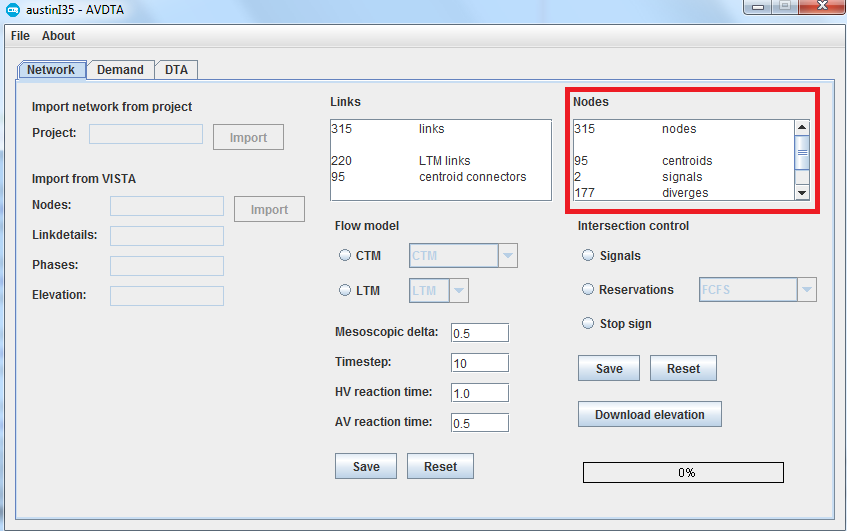
\includegraphics[width=0.8\textwidth]{images/nodes1.png}
\end{center}

The next panel controls intersections. Selecting an intersection control, then pressing the ``save'' button, will result in all intersections converted to the specified intersection control.
\begin{center}
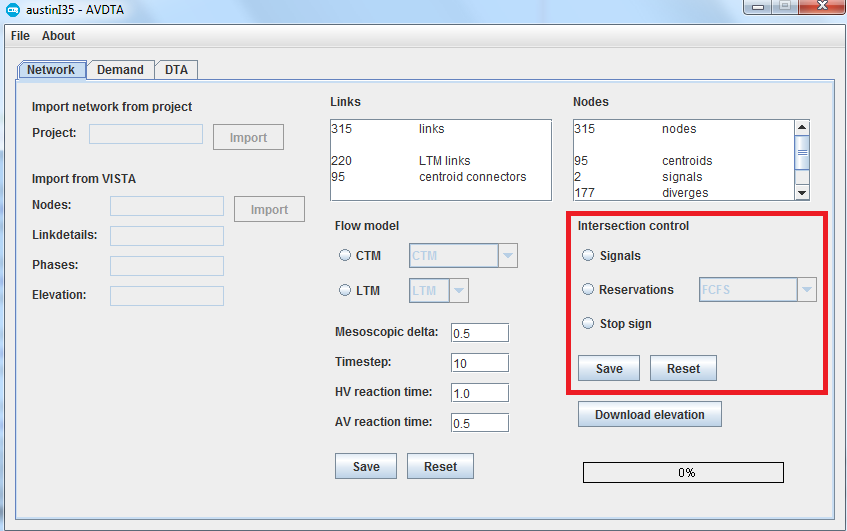
\includegraphics[width=0.8\textwidth]{images/nodes2.png}
\end{center}

The final panel will attempt to download elevation data from the Google Maps API. This will only affect nodes for which the elevation is 0. This requires a connection to the internet. The download may take some time because a delay between requests is necessary to avoid being rejected as a DOS attack. In addition, the Google Maps API may limit the number of requests per day. If the process exits with an error, restart it later. It will save progress and continue from where it left off.
\begin{center}
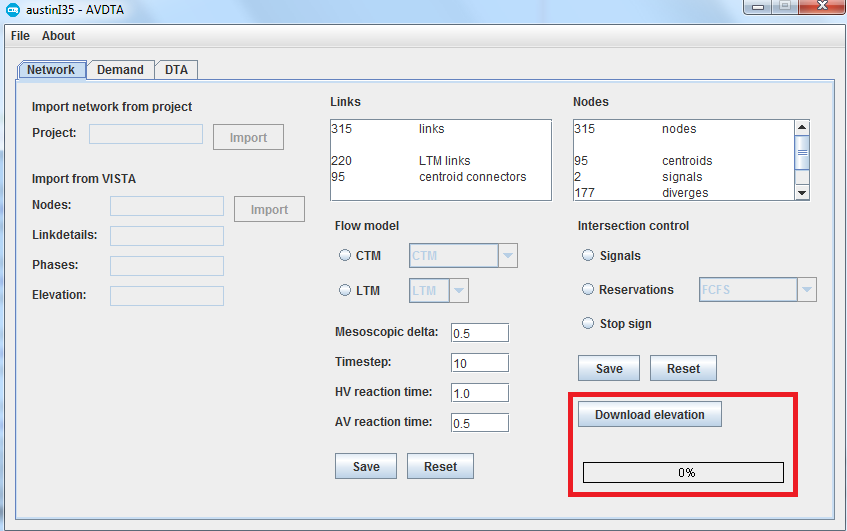
\includegraphics[width=0.8\textwidth]{images/nodes3.png}
\end{center}





\section{Links}
\label{sec:links}

\subsection{\texttt{links.txt}}

Each line in the \texttt{links.txt} file corresponds to a link in the network. The \texttt{links.txt} file has columns
\begin{center}
\begin{tabular}{ccccccccc}
\hline
id & type & source & dest & length & ffspd & w & capacity & num\_lanes \\\hline
\end{tabular}
\end{center}
\paragraph*{id} The id of the link. Each link must have an unique, positive id, but the ids do not have to be consecutive.
\paragraph*{type} This determines the flow model used for the link. The possible types are
\begin{center}
\begin{tabular}{lcl}
\hline Flow model & Type & Description\\\hline
CTM & 100 & Multiclass CTM~\cite{levin2016multiclass} \\
& 102 & CTM with DLR~\cite{levin2016cell}\\
& 103 & CTM with shared transit lane\\\hline
LTM & 200 & Standard LTM~\cite{yperman2005link, yperman2007link}\\
& 205 & LTM with CACC\\\hline
Centroid connector & 1000 & Link between a centroid and a node\\\hline
\end{tabular}
\end{center}
Standard CTM is achieved through type 100 with HVs.
\paragraph*{source} The id of the source node.
\paragraph*{dest} The id of the destination node.
\paragraph*{length} The length of the link, in feet. 
\paragraph*{ffspd} The free flow speed of the link, in miles per hour. Note that the free flow travel time is rounded up to the nearest time step.
\paragraph*{w} The congested wave speed of the link, in miles per hour. For LTM links, the free flow speed, capacity, and congested wave speed must be consistent as the fundamental diagram is over-determined. This is not an issue with CTM because CTM accepts a trapezoidal fundamental diagram. A typical value is half of the free flow speed.
\paragraph*{capacity} The capacity \textit{per lane} for the link, in vehicles per hour.
\paragraph*{num\_lanes} The number of lanes on the link. This affects the total capacity as well as intersection dynamics.

Note that for centroid connectors, the free flow travel time does not depend on the length and free flow speed, but is a constant 1 time step. Also, centroid connectors are not restricted by wavespeed or capacity limitations. 

With CTM, the minimum number of cells per link is two. This means the minimum free flow travel time is two time steps.

\subsection{GUI}

The center panel of the ``networks'' tab is used to interact with links. The uppermost text area displays information about the network, including the number of total links, and the number of links of various types.
\begin{center}
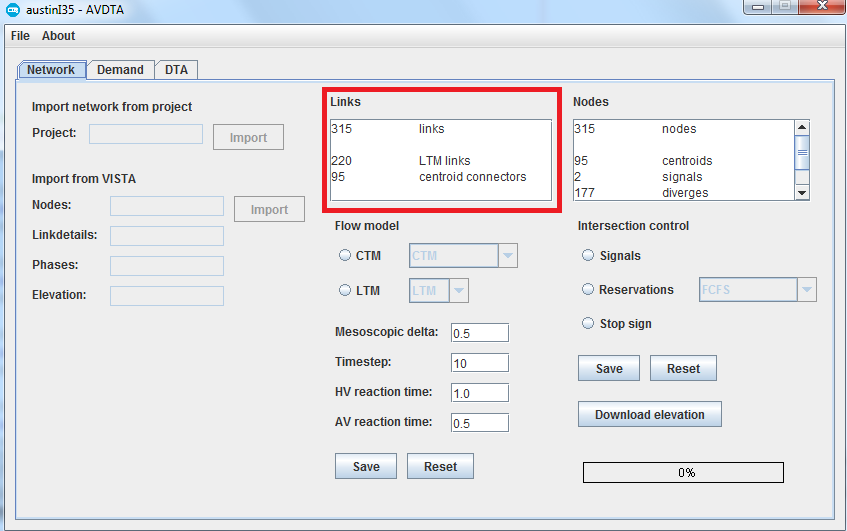
\includegraphics[width=0.8\textwidth]{images/links1.png}
\end{center}

The lower panel provides an interface for modifying the link flow model and network options. Selecting the ``CTM'' or ``LTM'' radio buttons, then pressing ``save'', will change all non-centroid connector links to the selected type. The ``mesoscopic delta'' field will set the congested wave speed to the specified fraction of the free flow speed for each link. The remaining text fields are network options (Section \ref{sec:options}).
\begin{center}
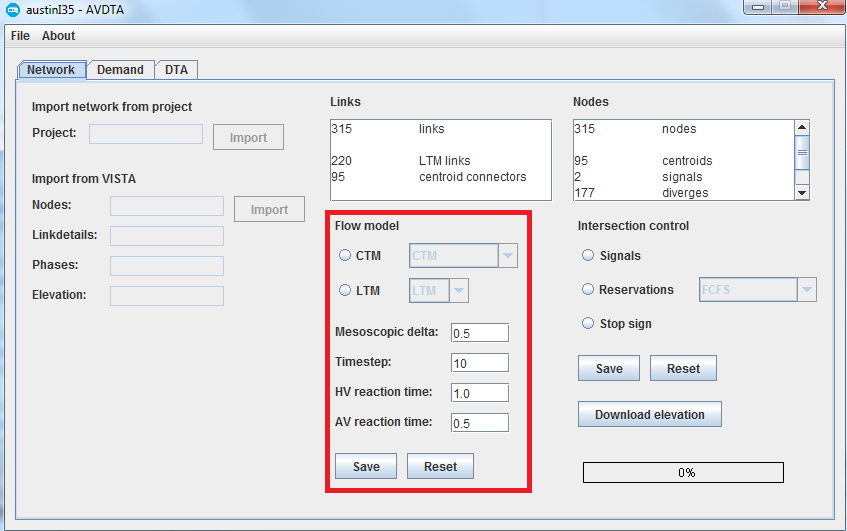
\includegraphics[width=0.8\textwidth]{images/links2.png}
\end{center}


\section{Import network}

The left hand side of the ``network tab'' contains an interface to import data from other sources. Note that using this interface will overwrite the network data of the project. There are two options. First, the network can be imported from any AVDTA project. This includes DTA projects and projects of other types. 
\begin{center}
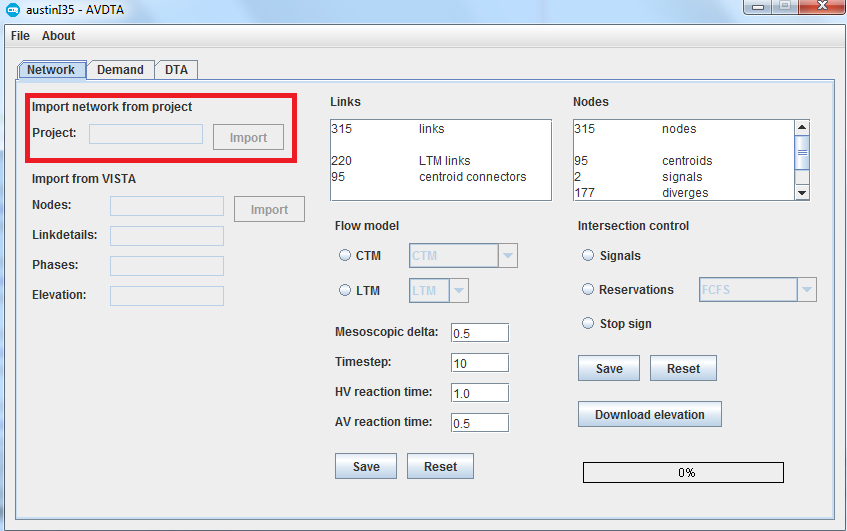
\includegraphics[width=0.8\textwidth]{images/network1.png}
\end{center}
Click on the text field to select a project file.

The second option is to import from VISTA. Copy the \texttt{nodes}, \texttt{linkdetails}, \texttt{phases}, and \texttt{signals} tables into text files, and select them by clicking on the text field. An optional elevation file can be used to fill node elevations. It is not required to import the network; if left blank, elevations of 0 will be used.
\begin{center}
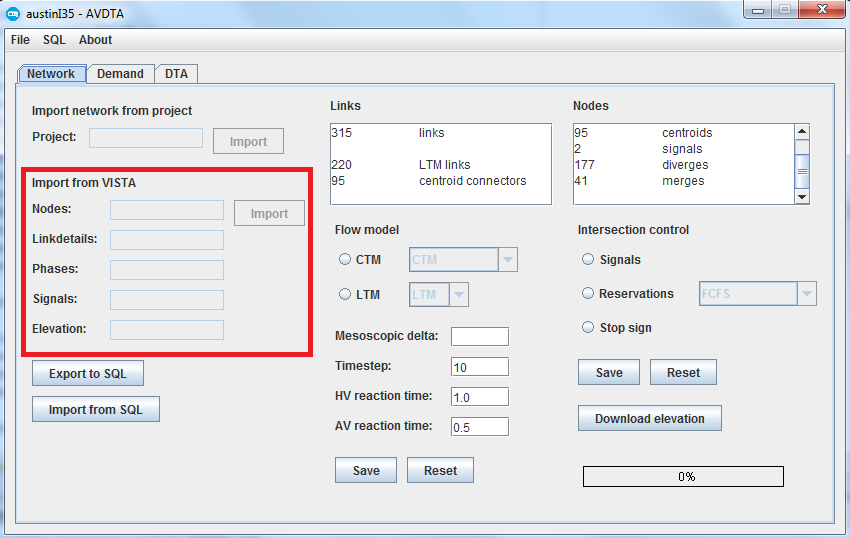
\includegraphics[width=0.8\textwidth]{images/network2.png}
\end{center}
AVDTA and VISTA use different file formats, so it is not recommended to copy VISTA tables into AVDTA directly.

The third option is to export or import data to/from SQL. This allows data to be manipulated within SQL, then returned to AVDTA in the appropriate format. To use SQL, the connection must first be set up (Section \ref{sec:setupsql}). Exporting will create and populate \texttt{nodes}, \texttt{linkdetails}, \texttt{phases}, \texttt{signals}, and \texttt{options} tables in the SQL database. Importing will copy the contents of these tables into AVDTA.
\begin{center}
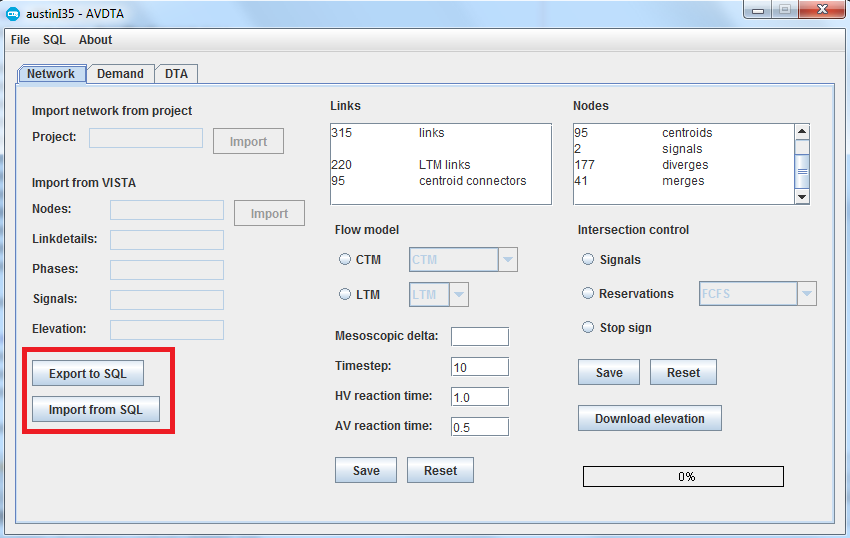
\includegraphics[width=0.8\textwidth]{images/sql2.png}
\end{center}

	
	% Demand structure
	%	Vehicles
	%	Static OD
	%	Dynamic OD
	%	Data files - include
	%	GUI - include
	%	Types - include
	% 	Import from VISTA
	\chapter{Demand}
\label{ch:demand}

\section{Introduction}

The demand specifies personal vehicle trips in terms of origins, destinations, and departure times. This chapter discusses the organization of the demand inputs to DTA. All related data files are contained within the \texttt{demand} subfolder of a project. The demand is specified through four files. The \texttt{static\_od.txt} file is a static (time-invariant) trip table that is representative of the static data available to many planning organizations. The \texttt{dynamic\_od.txt} file is a dynamic trip table that specifies the number of trips per \textit{assignment interval} (AST). The \texttt{demand\_profile.txt} file specifies the weight, start time, and duration of each AST. The \texttt{demand.txt} file contains a list of discrete vehicles, each with a specific origin, destination, and departure time. The \texttt{dynamic\_od.txt} file can be generated from the \texttt{static\_od.txt} and the \texttt{demand\_profile.txt} files. The \texttt{demand.txt} file can be generated from the \texttt{dynamic\_od.txt} file and the \texttt{demand\_profile.txt} file.
Vehicle types (i.e. HV, AV, etc.) are specified in the \texttt{static\_od.txt}, \texttt{dynamic\_od.txt}, and \texttt{demand.txt} files. The AVDTA GUI includes methods to generate the \texttt{dynamic\_od.txt} and \texttt{demand.txt} files given appropriate inputs.

\section{Files} 

\subsection{\texttt{static\_od.txt}}
\label{sec:staticod}

The \texttt{static\_od.txt} file is a time-invariant trip table. Each line indicates the number of trips of some type between some origin and destination. The columns are 
\begin{center}
\begin{tabular}{ccccc}
\hline
id & type & origin & destination & demand\\\hline
\end{tabular}
\end{center}
\paragraph*{id} An unique id for the trip table entry. Ids do not have to be consecutive, but must be unique and positive.
\paragraph*{type} The type indicates the type of vehicle, including the driver, engine, and vehicle behavior. The options for types are indicated below:
\begin{center}
\begin{tabular}{lcl}
\hline
Category & type & description \\\hline
Driver & 10 & HV \\
 & 20 & AV\\\hline
Engine & 1 & ICV \\
& 2 & BEV\\\hline
Behavior & 100 & personal vehicle (UE routing)\\
& 500 & transit (fixed route)\\\hline
\end{tabular}
\end{center}
A valid type is the sum of a driver type, an engine type, and a vehicle behavior. Typical types are 111 for HVs and 121 for AVs.

\paragraph*{origin, destination} These are ids of origin and destination zones in the network (see Section \ref{sec:nodes}).
\paragraph*{demand} A floating point number indicating the number of trips of the specified type from the origin to the destination. Duplicate entries (in terms of type, origin, and destination) are accepted.

\subsection{\texttt{dynamic\_od.txt}}
\label{sec:dynamicod}

The \texttt{dynamic\_od.txt} file is like the \texttt{static\_od.txt} file, but with the addition of an AST. Each line The columns are
\begin{center}
\begin{tabular}{cccccc}
\hline
id & type & origin & destination & ast & demand\\\hline
\end{tabular}
\end{center}
\paragraph*{ast} This is the id of an AST from the \texttt{demand\_profile.txt} file (Section \ref{sec:demandprofile}).

The remainder of the columns are the same as in the \texttt{static\_od.txt} file (Section \ref{sec:staticod}). The ids in \texttt{dynamic\_od.txt} do not need to correspond to the ids in \texttt{static\_od.txt}. The \texttt{dynamic\_od.txt} file can be generated within AVDTA from the \texttt{static\_od.txt} and \texttt{demand\_profile.txt} files. The distribution of flow over ASTs is determined by the weights in the \texttt{demand\_profile.txt} file.

\subsection{\texttt{demand\_profile.txt}}
\label{sec:demandprofile}

The \texttt{demand\_profile.txt} file specifies the ASTs. Each line is an individual AST. The columns are
\begin{center}
\begin{tabular}{cccc}
\hline
id & weight & start & duration \\\hline
\end{tabular}
\end{center}
\paragraph*{id} The id must be positive and unique, but does not need to be consecutive.
\paragraph*{weight} This is the proportion of total flow departing within this AST. Proportions will be scaled to sum to 1 if necessary.
\paragraph*{start} This is the starting time of the AST, measured in seconds from the beginning of the simulation period.
\paragraph*{duration} This is the duration of the AST. A typical value is 900 (s).


\subsection{\texttt{demand.txt}}
Each line in the \texttt{demand.txt} file is an individual vehicle trip. The columns are
\begin{center}
\begin{tabular}{cccccc}
\hline
id & type & origin & dest & dtime & vot \\\hline
\end{tabular}
\end{center}
\paragraph*{id} The unique vehicle id. Ids must be positive and unique but do not have to be consecutive.
\paragraph*{type} The vehicle type (see Section \ref{sec:staticod} for a list of types).
\paragraph*{origin, dest} The ids of the origin and destination zones for the vehicle (see Section \ref{sec:nodes}).
\paragraph*{dtime} The departure time of the vehicle, measured in seconds from the start of the simulation period.
\paragraph*{vot} The value of time of the vehicle. This is used in certain control policies, such as auctions for reservations. Values of time must be non-negative.


\section{GUI}
This section describes how to interact with the demand through the AVDTA GUI. The ``demand'' tab contains all demand interactions. 

\subsection{Import demand}
The left hand side contains options to import demand from other sources. The first option is to import the demand from another DTA project. This will copy all demand files from the specified project, overwriting any demand files in the current project. Click on the text field to select the project.
\begin{center}
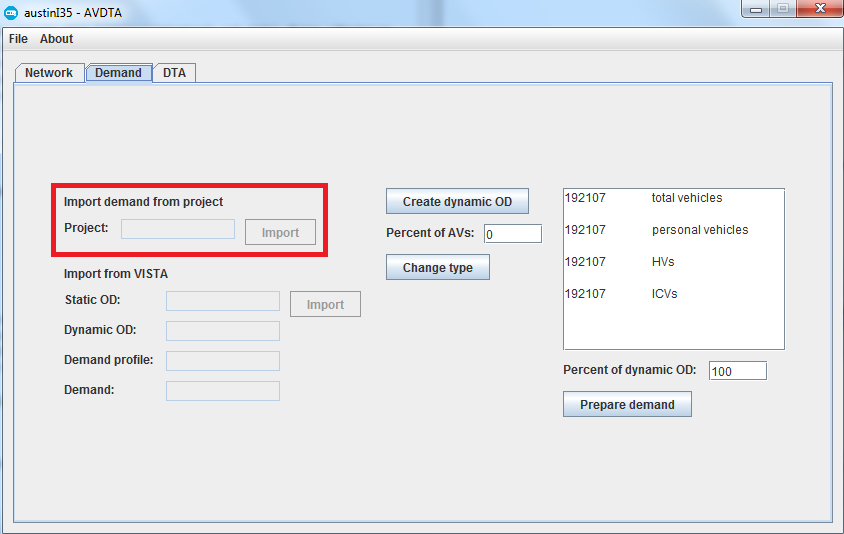
\includegraphics[width=0.8\textwidth]{images/demand1.png}
\end{center}

The second option is to import demand from VISTA. This requires the \texttt{static\_od}, \texttt{dynamic\_od}, \texttt{demand\_profile}, and \texttt{demand} tables from the VISTA database. Copy them into text files, and select the text files by clicking on the text fields. Note that the file format of AVDTA is not the same as the file format of VISTA, so using the GUI to import demand is recommended.
\begin{center}
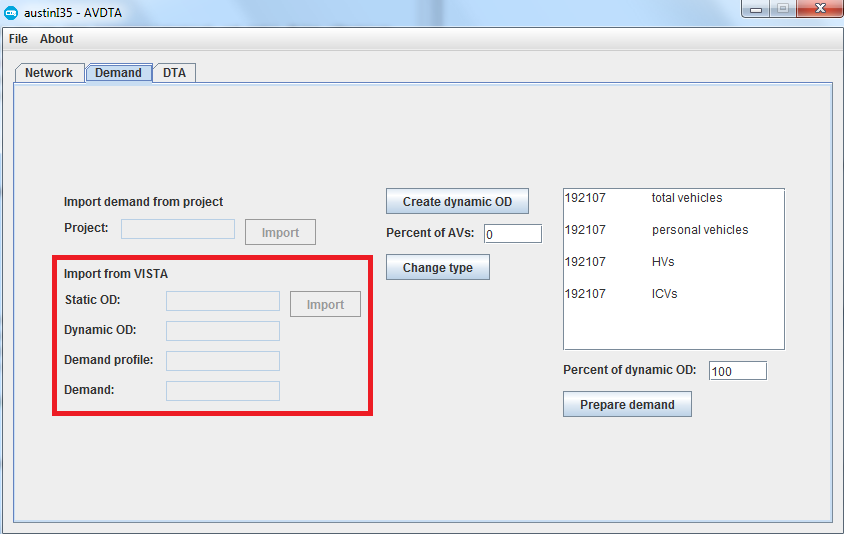
\includegraphics[width=0.8\textwidth]{images/demand2.png}
\end{center}

The third option is to export or import data to/from SQL. This allows data to be manipulated within SQL, then returned to AVDTA in the appropriate format. To use SQL, the connection must first be set up (Section \ref{sec:setupsql}). Exporting will create and populate \texttt{static\_od}, \texttt{dynamic\_od}, \texttt{demand\_profile}, and \texttt{demand}, tables in the SQL database. Importing will copy the contents of these tables into AVDTA.
\begin{center}
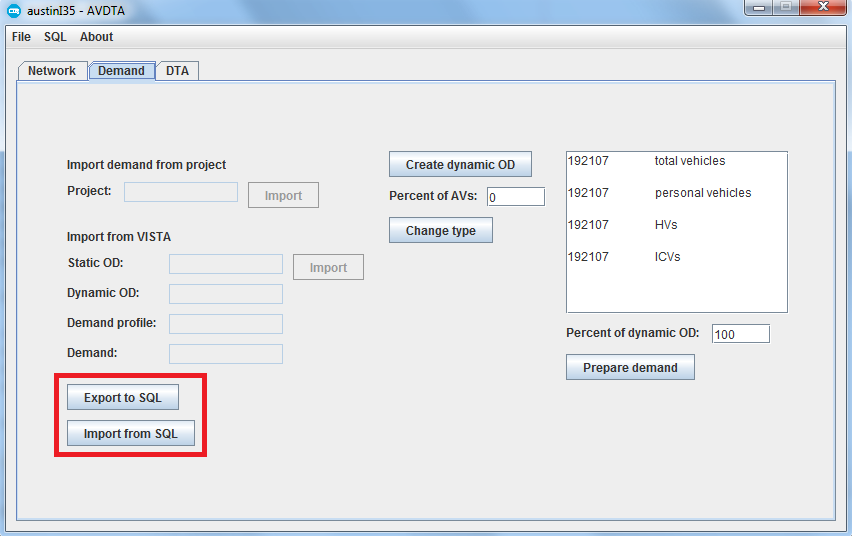
\includegraphics[width=0.8\textwidth]{images/sql3.png}
\end{center}


\subsection{Creating demand}
The middle section includes options to change the \texttt{dynamic\_od.txt} file. The first button will generate the \texttt{dynamic\_od.txt} file based on the \texttt{static\_od.txt} and the \texttt{demand\_profile.txt} files, as discussed in Section \ref{sec:dynamicod}. 
\begin{center}
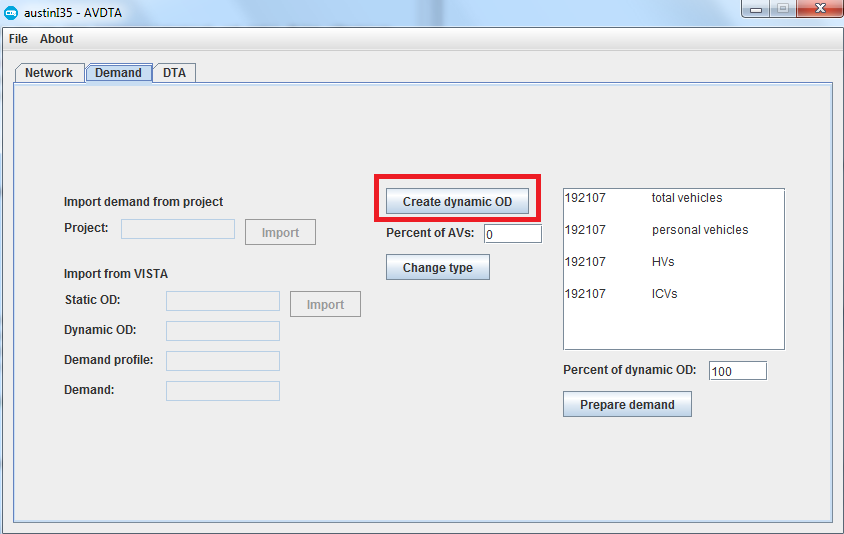
\includegraphics[width=0.8\textwidth]{images/demand3.png}
\end{center}

The second option will change the type of vehicles to 111 for HVs or 121 for AVs (see Section \ref{sec:staticod} for types) in the \texttt{dynamic\_od.txt} file based on the specified percent of AVs. 
\begin{center}
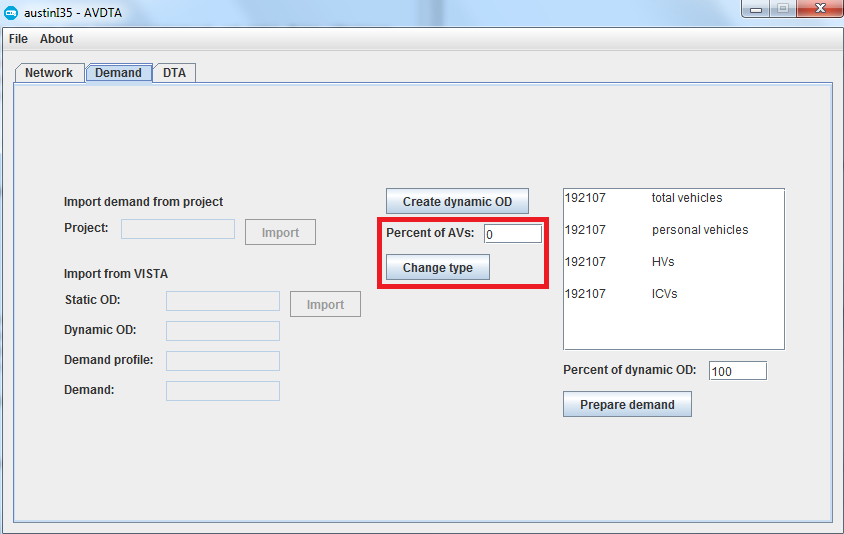
\includegraphics[width=0.8\textwidth]{images/demand3b.png}
\end{center}

The right hand side describes the individual vehicle trips. The text area lists the total numbers of vehicles, then breaks down the numbers of vehicles by type (driver, engine, and behavior). Click the ``prepare demand'' button to generate the \texttt{demand.txt} file from the \texttt{dynamic\_od.txt} and \texttt{demand\_profile.txt} files. You can also scale the percent of demand. 

Preparing demand uses a random number generator when the number of trips is not an integer. If $d$ is the number of vehicle trips in \texttt{dynamic\_od.txt}, prepare demand will create either $\lfloor d\rfloor$ or $\lceil d\rceil$ trips depending on the outcome of the random number generator.
\begin{center}
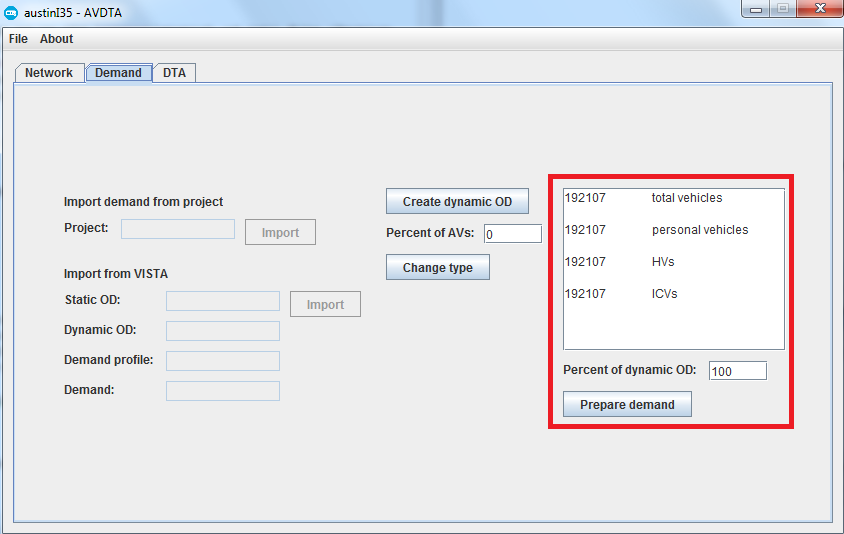
\includegraphics[width=0.8\textwidth]{images/demand4.png}
\end{center}


	
	% DTA
	
	\addcontentsline{toc}{chapter}{References}
	\bibliography{MWL}
	\bibliographystyle{acm}
	
\end{document}